% !TeX root=../main.tex

\chapter*{پاسخ سوالات سری چهارم}

% دستور زیر باعث عدم‌نمایش شماره صفحه در اولین صفحهٔ این فصل می‌شود.
%\thispagestyle{empty}
\section*{ پاسخ سوال 1}
\subsection*{بخش یکم}

در سوال اول با توجه به معادلات حالت سیستم که به صورت زیر داده شده است، می توانیم درکی از سیستم به دست بیاوریم:]
\[
\begin{bmatrix}
	\dot{x}_1 \\ \dot{x}_2 \\ \dot{x}_3 \\ \dot{x}_4
\end{bmatrix}
=
\begin{bmatrix}
	0 & 1 & 0 & 0 \\
	0 & -\frac{c_S}{M_S} & \frac{k_S}{M_S} & \frac{c_S}{M_S} \\
	0 & 0 & 1 & 0 \\
	-\frac{k_U}{M_U} & \frac{c_S}{M_U} & \frac{k_S + k_U}{M_U} & \frac{-c_S + c_U}{M_U}
\end{bmatrix}
\begin{bmatrix}
	x_1 \\ x_2 \\ x_3 \\ x_4
\end{bmatrix}
+
\begin{bmatrix}
	0 \\ \frac{c_S c_U}{M_S M_U} \\ -\frac{c_U}{M_U} \\ \frac{c_U}{M_U}\left(\frac{k_U}{c_U} - \frac{c_S}{M_U} - \frac{c_U}{M_U}\right)
\end{bmatrix}
d
+
\begin{bmatrix}
	0 \\ \frac{1}{M_S} \\ 0 \\ -\frac{1}{M_U}
\end{bmatrix}
u
\]

\[
\begin{bmatrix}
	y_1 \\ y_2 \\ y_3
\end{bmatrix}
=
\begin{bmatrix}
	1 & 0 & 0 & 0 \\
	0 & 1 & 0 & 0 \\
	0 & 0 & 1 & 0
\end{bmatrix}
\begin{bmatrix}
	x_1 \\ x_2 \\ x_3 \\ x_4
\end{bmatrix}
+
\begin{bmatrix}
	0 \\ 0 \\ 0
\end{bmatrix}
d
+
\begin{bmatrix}
	0 \\ 0 \\ 0
\end{bmatrix}
u
\]

مشاهده می شود که سیستم دارای چهار حالت و سه خروجی مشاهده پذیر است.
ساختار کنترلی پیش بین خطی برای این سوال به صورت زیر طراحی می شود.
\begin{figure}[H]
	\centering
	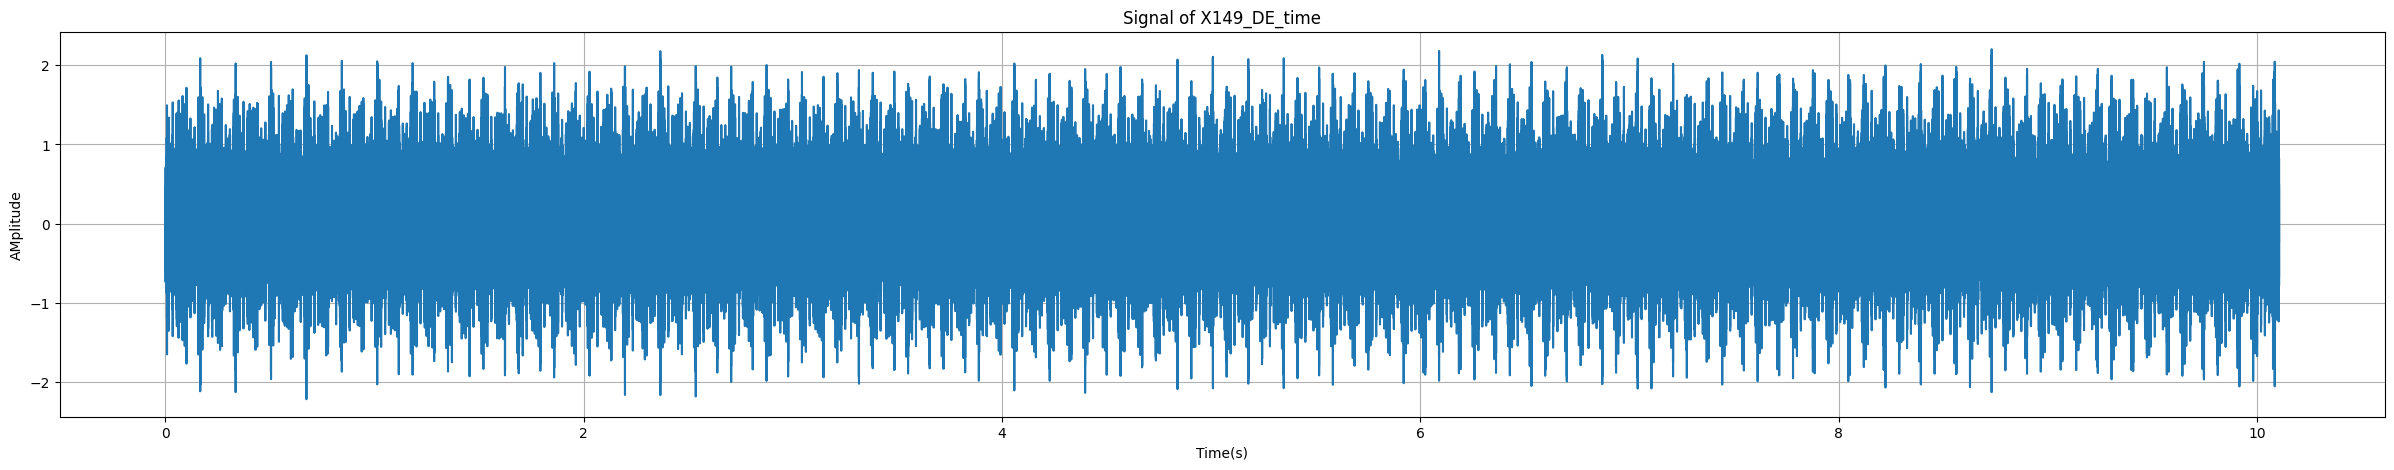
\includegraphics[width=1\linewidth]{../img/1}
	\caption{بلوک دیاگرام LMPC}
	\label{fig:1}
\end{figure}
لازم به ذکر است که با توجه به محدودیت های متلب برای ابعاد ورودی ها، خروجی ها و حالت های سیستم، چهار خروجی برای سیستم تعریف شده است، اما خروجی چهارم که نیازی نیست در نظر گرفته شود با مقدار 0 در نظر گرفته می شود.
معادلات سیستم را به صورت زیر در یک سیستم تعریف می کنیم.
\begin{figure}[H]
	\centering
	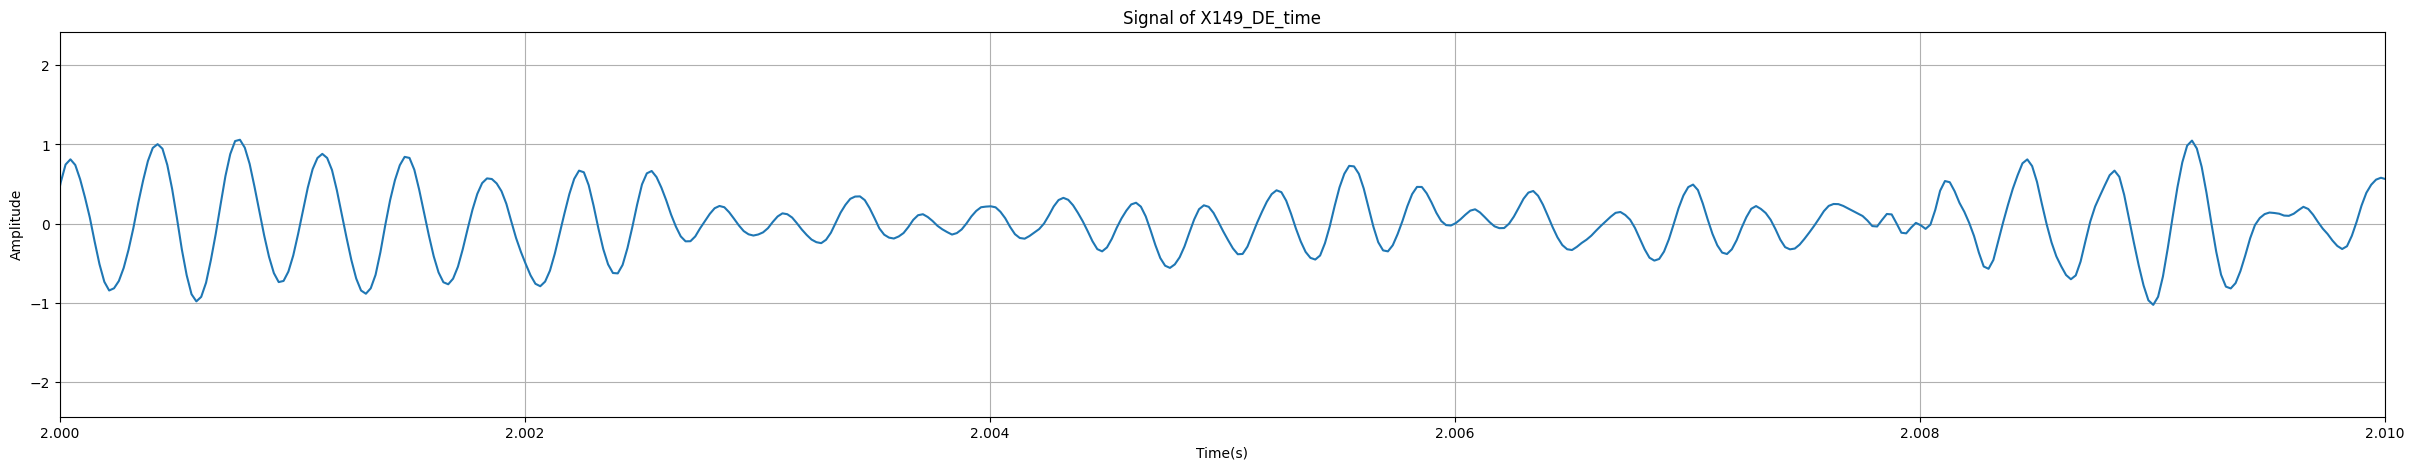
\includegraphics[width=1\linewidth]{../img/2}
	\caption{کد پلنت سیستم}
	\label{fig:2}
\end{figure}
همچنین، اغتشاش وارد شده به سیستم توسط کد زیر ایجاد می شود.

\begin{figure}[H]
	\centering
	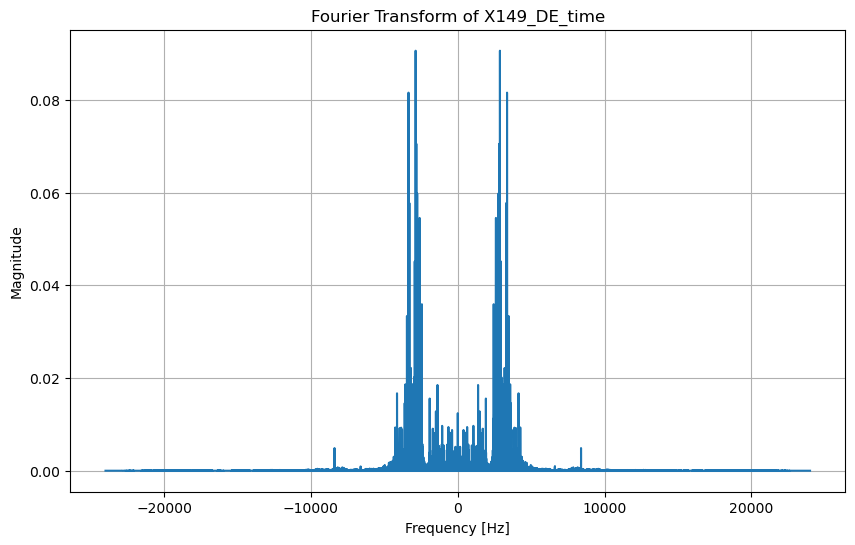
\includegraphics[width=0.4\linewidth]{../img/3}
	\caption{اغتشاش}
	\label{fig:3}
\end{figure}
در ادمه، با طراحی کنترلر MPC برای این سیستم با تنظیمات زیر، می توانیم نتایج به دست آمده از سیستم را مشاهده کنیم:

\begin{figure}[H]
	\centering
	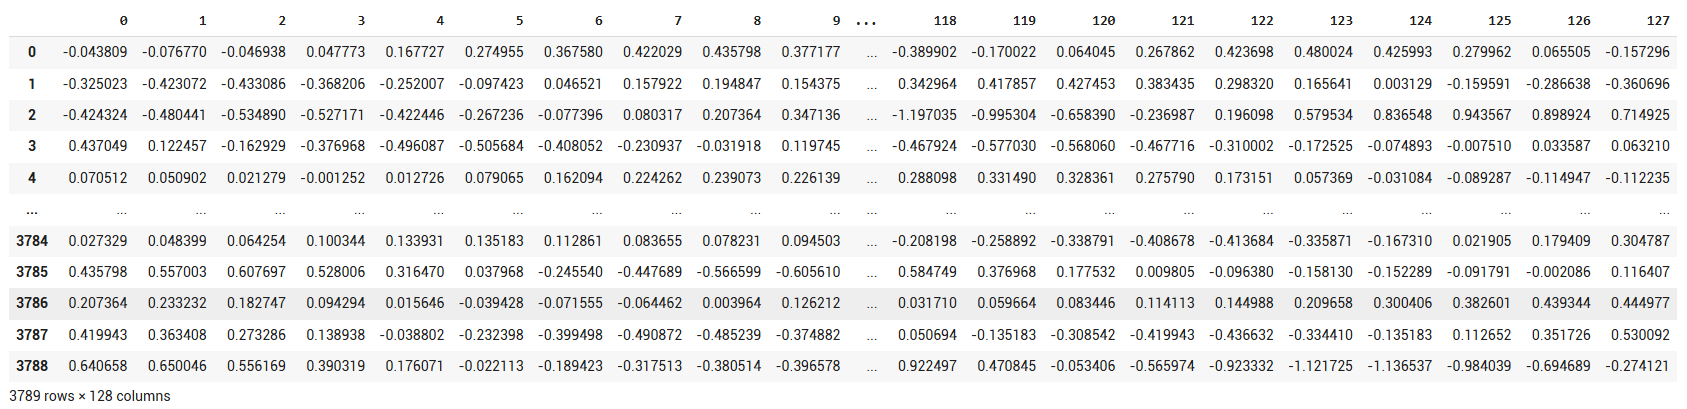
\includegraphics[width=1\linewidth]{../img/4}
	\caption{LMPC design}
	\label{fig:4}
\end{figure}
همچنین باید توجه شود که قید هایی برای حالت اول سیستم در نظر گرفته شده است تا مقدار آن از 1 بیشتر نشود. 

\begin{figure}[H]
	\centering
	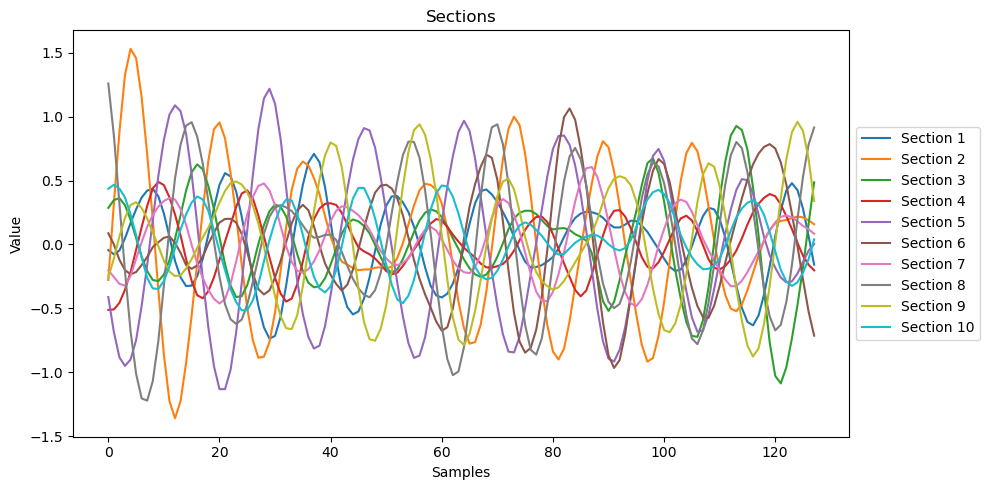
\includegraphics[width=1\linewidth]{../img/5}
	\caption{LMPC constraints configuration}
	\label{fig:5}
\end{figure}
با استفاده از سیستم تعریف شده، پاسخ های سیستم به صورت زیر به دست می آید.

\begin{figure}[H]
	\centering
	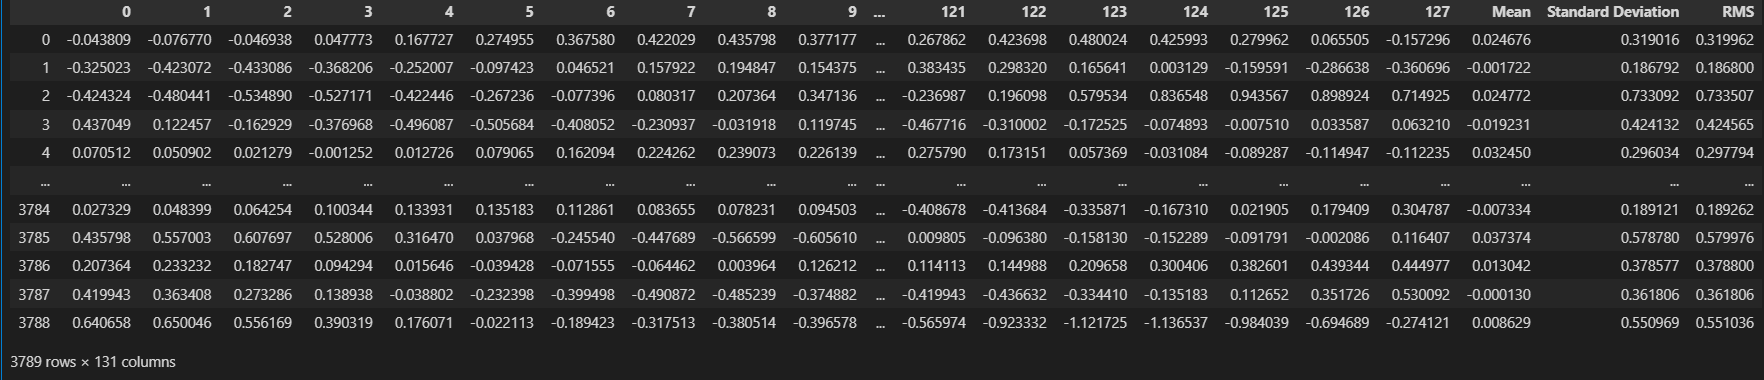
\includegraphics[width=1\linewidth]{../img/6}
	\caption{LMPC states output}
	\label{fig:6}
\end{figure}
همچنین نمودار تلاش کنترلی سیستم یه صورت زیر به دست می آید.

\begin{figure}[H]
	\centering
	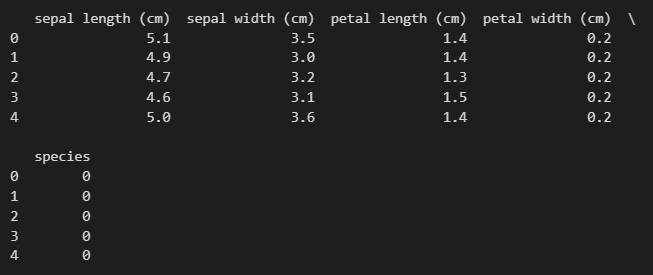
\includegraphics[width=1\linewidth]{../img/7}
	\caption{LMPC control effort}
	\label{fig:7}
\end{figure}

با در اختیار داشتن نتایج به دست آمده و به منظور تحلیل این نتایج، کنترلر PID نیز برای سیستم طراحی و بررسی می شود. دیاگرام این سیستم به شرح زیر خواهد بود:

\begin{figure}[H]
	\centering
	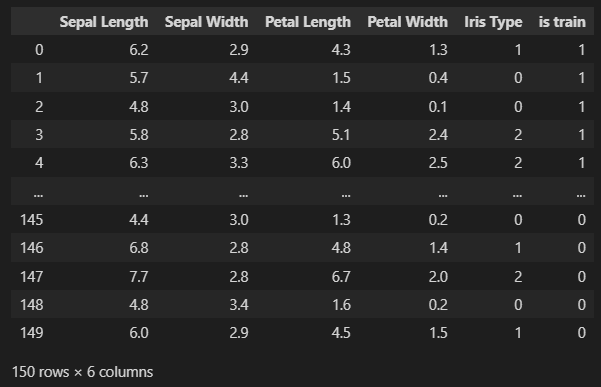
\includegraphics[width=1\linewidth]{../img/8}
	\caption{PID diagram}
	\label{fig:8}
\end{figure}

لازم به ذکر است که برای این سیستم، تنها حالت اول به عنوان خروجی سیستم در نظر گرفته شده است. پاسخ سیستم به صورت زیر به دست می آید و مشاهده می شود که می تواند به خوبی اغتشاش وارد شده را رفع کند. اما با در نظر گرفتن ضرایب PID و همچنین نمودار تلاش کنترلی مشاهده می شود که در نهایت این کنترلر در سیستم های واقعی قابل پیاده سازی نمی باشد.

\begin{figure}[H]
	\centering
	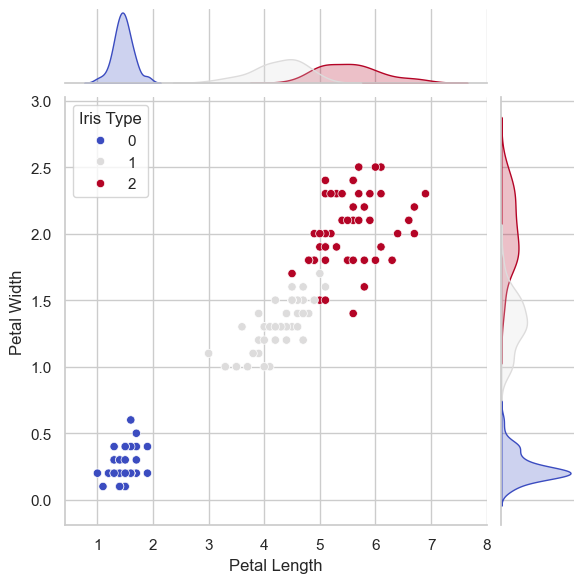
\includegraphics[width=1\linewidth]{../img/9}
	\caption{PID control effort}
	\label{fig:9}
\end{figure}

\begin{figure}[H]
	\centering
	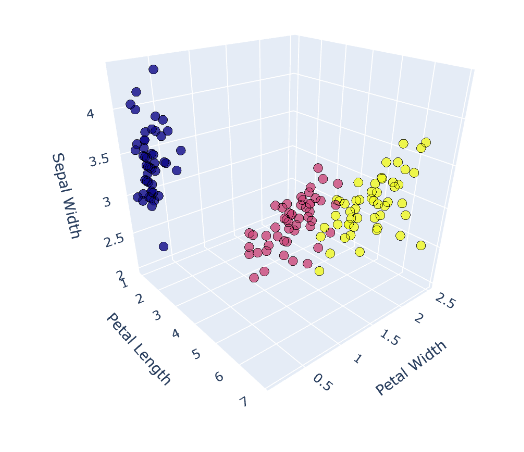
\includegraphics[width=0.7\linewidth]{../img/10}
	\caption{}
	\label{fig:10}
\end{figure}

\begin{figure}[H]
	\centering
	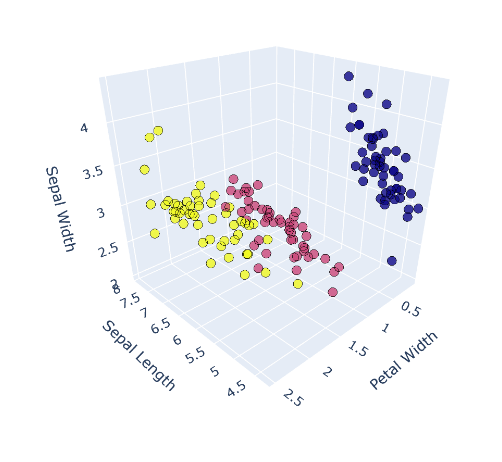
\includegraphics[width=1\linewidth]{../img/11}
	\caption{PID state1 output}
	\label{fig:11}
\end{figure}

در اینجا با در نظر گرفتن نتایج به دست آمده از MPC و PID می توانیم مقایسه ای در عملکرد آنها داشته باشیم.
نتایج به دست امده از خروجی کنترلی حالت اول با این دو کنترلر و تلاش کنترلی برای رفع آن به صورت زیر خواهد بود.

\begin{figure}[H]
	\centering
	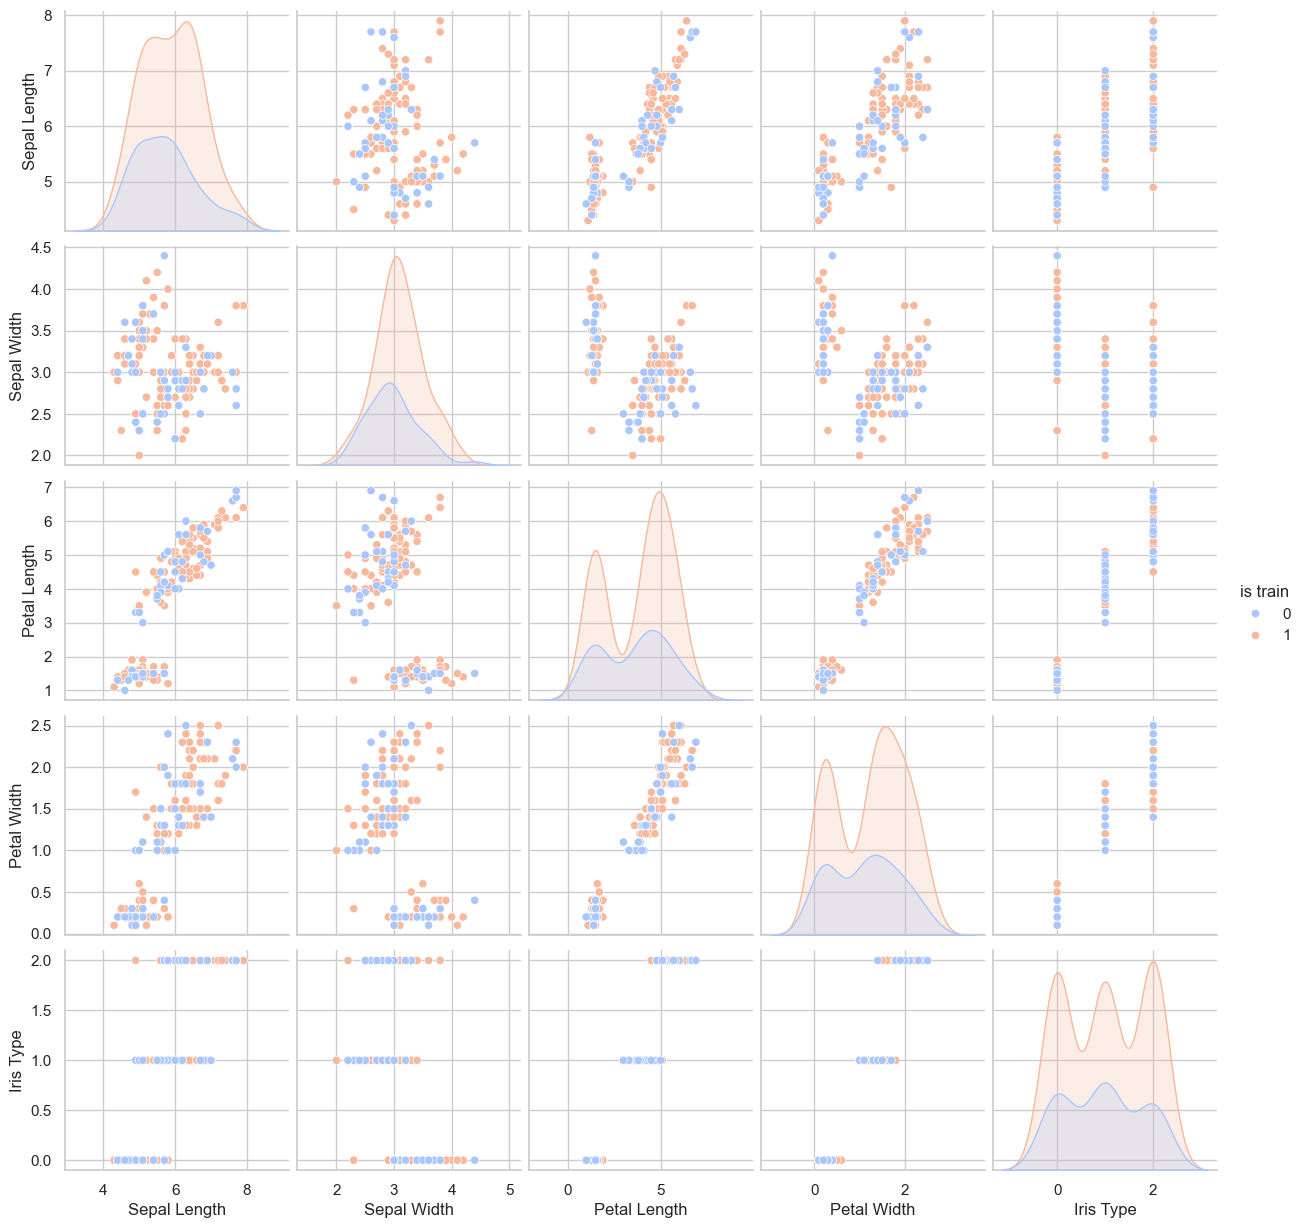
\includegraphics[width=1\linewidth]{../img/13}
	\caption{LMPC state1 output}
	\label{fig:13}
\end{figure}

\begin{figure}[H]
	\centering
	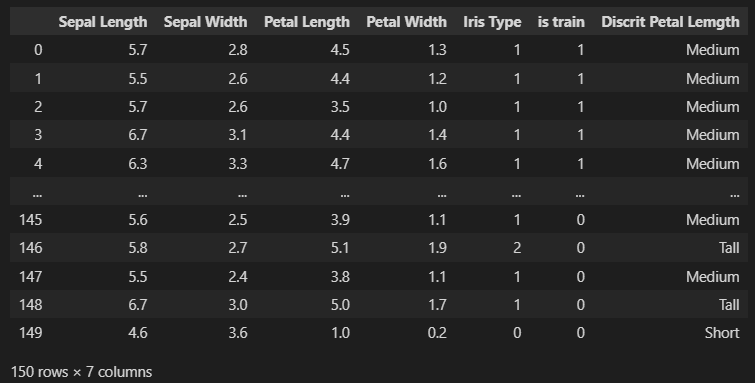
\includegraphics[width=1\linewidth]{../img/14}
	\caption{PID vs LMPC control effort}
	\label{fig:14}
\end{figure}

همچنین مقادیر RMSE برای این دو کنترلر در دو حالت مورد نظر به صورت زیر به دست می آید.

\begin{figure}[H]
	\centering
	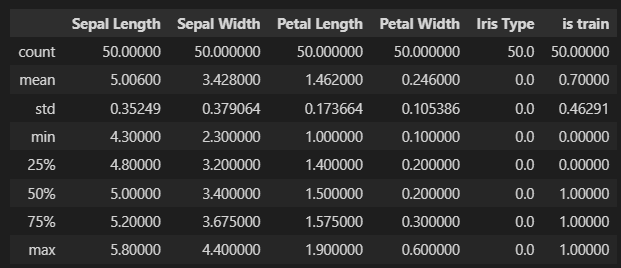
\includegraphics[width=1\linewidth]{../img/15}
	\caption{PID vs LMPC RMSE of states 1 and 3}
	\label{fig:15}
\end{figure}
نتایج به دست آمده نشان می ددهد که مقادیر RMSE برای کنترلر MPC بیشتر از کنترلر PID است. 
همچنین، مقدار RMSE برای ورودی کنترلرها به صورت زیر خواهد بود:

\begin{figure}[H]
	\centering
	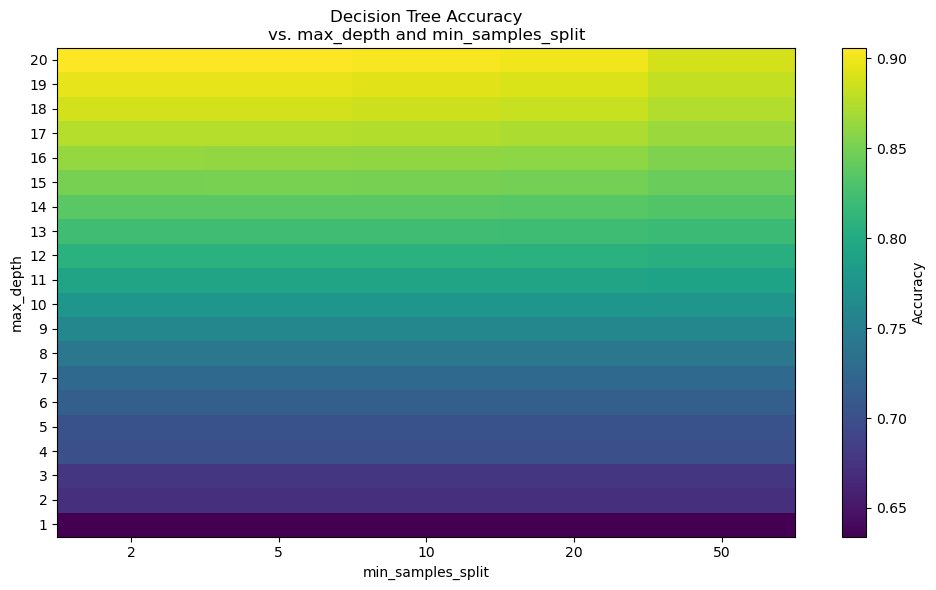
\includegraphics[width=1\linewidth]{../img/16}
	\caption{PID vs LMPC control effort RMSE}
	\label{fig:16}
\end{figure}
در نتیجه دیاگرام های سیستم ها با تجه به تغییرات اعمال شده به صورت زیر برای دو کنترلر خواهد بود.

\begin{figure}[H]
	\centering
	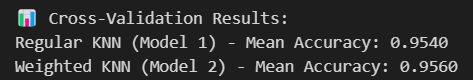
\includegraphics[width=1\linewidth]{../img/17}
	\caption{کنترلر Tube}
	\label{fig:17}
\end{figure}

\begin{figure}[H]
	\centering
	\includegraphics[width=1\linewidth]{../img/18}
	\caption{کنترلر LMPC}
	\label{fig:18}
\end{figure}

\subsection*{بخش دوم}
در این بخش، با افزودن یک کنترلر PID به MPC و تشکیل یک کنترلر $Tube MPC$، مجددا نتایج را بررسی می کنیم. بنابراین، ساختار سیستم طراحی شده به صورت زیر خواهد بود:

\begin{figure}[H]
	\centering
	\includegraphics[width=1\linewidth]{../img/19}
	\caption{کنترلر LMPC}
	\label{fig:19}
\end{figure}
در ادامه، با تنظیم مجدد کنترلر MPC و PID، کنترلر ها را مجددا طراحی می کنیم. تنظیم های کنترلر PID به صورت زیر خواهد بود.
\begin{figure}[H]
	\centering
	\includegraphics[width=1\linewidth]{../img/20}
	\caption{}
	\label{fig:20}
\end{figure}

\begin{figure}[H]
	\centering
	\includegraphics[width=1\linewidth]{../img/21}
	\caption{}
	\label{fig:21}
\end{figure}
تنظیمات MPC به صورت زیر خواهد بود:

\begin{figure}[H]
	\centering
	\includegraphics[width=1\linewidth]{../img/22}
	\caption{}
	\label{fig:22}
\end{figure}

% TODO: \usepackage{graphicx} required
\begin{figure}[h!]
	\centering
	\includegraphics[width=1\linewidth]{../img/23}
	\caption{}
	\label{fig:23}
\end{figure}

% TODO: \usepackage{graphicx} required
\begin{figure}[H]
	\centering
	\includegraphics[width=1\linewidth]{../img/24}
	\caption{}
	\label{fig:24}
\end{figure}

% TODO: \usepackage{graphicx} required
\begin{figure}[H]
	\centering
	\includegraphics[width=1\linewidth]{../img/25}
	\caption{}
	\label{fig:25}
\end{figure}

\newpage
\subsection*{بخش سوم}
در قسمت بعد، سیستم را با پیاده سازی کنترلر $Explicit MPC$ به جای کنترلر LMPC کنترل می کنیم. 
برای این کار با استفاده از دستورات $generateExplicitRange$،
$generateExplicitOptions$ و 
$generateExplicitMPC$
کنترلر MPC طراحی شده را با شرایط زیر به کنترلر EMPC تبدیل می کنیم. 
% TODO: \usepackage{graphicx} required
\begin{figure}[H]
	\centering
	\includegraphics[width=1\linewidth]{../img/26}
	\caption{}
	\label{fig:26}
\end{figure}

در اینجا لازم به ذکر است که استفاده از افق های پیش بینی و کنترل مورد استفاده در LMPC (افق پیش بین: 100، افق کنترل 30) برای کنترلر EMPC بسیار زیاد بوده و تعداد نواحی بسیار زیادی را ایجاد میکند که برای پیاده سازی، امکان پذیر نیست. بنابراین، پارامتر های این کنترلر به مقادیر زیر تغییر کرده اند.
افق پیش بین: 30
افق کنترل: 3

با اجرای برنامه، خروجی کنترلر به صورت زیر به دست می اید و مشاهده می شود که عملکردی مشابه با کنترلر LMPC دارد. 

\begin{figure}[H]
	\centering
	\includegraphics[width=0.7\linewidth]{../img/27}
	\caption{}
	\label{fig:27}
\end{figure}

مقادیر RMSE محاسبه شده برای این مدل به صورت زیر خواهد بود.
% TODO: \usepackage{graphicx} required
\begin{figure}[H]
	\centering
	\includegraphics[width=0.7\linewidth]{../img/28}
	\caption{ٍ}
	\label{fig:28}
\end{figure}

در نهایت، به مقایسه ی نتایج به دست آمده از کنترلر های ارائه شده برای این سیستم خواهیم پرداخت.

مقایسه حالت اول:
% TODO: \usepackage{graphicx} required
\begin{figure}[H]
	\centering
	\includegraphics[width=0.7\linewidth]{../img/29}
	\caption{}
	\label{fig:29}
\end{figure}

مقایسه حالت دوم:
% TODO: \usepackage{graphicx} required
\begin{figure}[H]
	\centering
	\includegraphics[width=0.7\linewidth]{../img/30}
	\caption{}
	\label{fig:30}
\end{figure}
مقایسه حالت سوم:
% TODO: \usepackage{graphicx} required
\begin{figure}[H]
	\centering
	\includegraphics[width=0.7\linewidth]{../img/31}
	\caption{}
	\label{fig:31}
\end{figure}
مقایسه تلاش کنترلی:
% TODO: \usepackage{graphicx} required
\begin{figure}[H]
	\centering
	\includegraphics[width=0.7\linewidth]{../img/32}
	\caption{}
	\label{fig:32}
\end{figure}


مقایسه RMSE حالت 1:
% TODO: \usepackage{graphicx} required
\begin{figure}[H]
	\centering
	\includegraphics[width=0.7\linewidth]{../img/33}
	\caption{}
	\label{fig:33}
\end{figure}

مقایسه RMSE حالت 3:
% TODO: \usepackage{graphicx} required
\begin{figure}[H]
	\centering
	\includegraphics[width=0.7\linewidth]{../img/34}
	\caption{}
	\label{fig:34}
\end{figure}

مقایسه RMSE کنترلر:
% TODO: \usepackage{graphicx} required
\begin{figure}[H]
	\centering
	\includegraphics[width=0.7\linewidth]{../img/35}
	\caption{}
	\label{fig:35}
\end{figure}

\subsection*{بخش چهارم}
در این بخش، یک کنترلر $Tube explicit MPC$ با اضافه کردن کنترلر PID به سیستم طراحی خواهد شد. ساختار دیاگرام این سیستم به صورت زیر است:
% TODO: \usepackage{graphicx} required
\begin{figure}[H]
	\centering
	\includegraphics[width=0.7\linewidth]{../img/36}
	\caption{}
	\label{fig:36}
\end{figure}

ضرایب PID مانند کنترلر $Tube MPC$ طراحی شده است و بلوک EMPC نیز با استفاده از تنظیمات نمایش داده شده در بخش قبل در دیاگرام قرار گرفته است.
پاسخ های به دست آمده از این سیستم در شکل زیر نمایش داده شده است.
% TODO: \usepackage{graphicx} required
\begin{figure}[H]
	\centering
	\includegraphics[width=0.7\linewidth]{../img/37}
	\caption{}
	\label{fig:37}
\end{figure}

همچنین نمودار تلاش کنترلی این سیستم به صورت زیر است:
% TODO: \usepackage{graphicx} required
\begin{figure}[H]
	\centering
	\includegraphics[width=0.7\linewidth]{../img/38}
	\caption{}
	\label{fig:38}
\end{figure}

و مقادیر RMSE به دست آمده برای این سیستم در شکل زیر نمایش داده شده است:
% TODO: \usepackage{graphicx} required
\begin{figure}[H]
	\centering
	\includegraphics[width=0.7\linewidth]{../img/39}
	\caption{}
	\label{fig:39}
\end{figure}
% TODO: \usepackage{graphicx} required
\begin{figure}[H]
	\centering
	\includegraphics[width=0.7\linewidth]{../img/40}
	\caption{}
	\label{fig:40}
\end{figure}

در پایان این بخش، به مقایسه ی نتایج به دست آمده از کنترلر TEMPC با کنترلر TMPC خواهیم پرداخت.
نمودار خروجی حالت اول سیستم با استفاده از این دو کنترلر به صورت زیر است:
% TODO: \usepackage{graphicx} required
\begin{figure}[H]
	\centering
	\includegraphics[width=0.7\linewidth]{../img/41}
	\caption{}
	\label{fig:41}
\end{figure}

همچنین، نمودار تلاش کنترلی برای این دو در شکل زیر نمایش داده شده است:
% TODO: \usepackage{graphicx} required
\begin{figure}[H]
	\centering
	\includegraphics[width=0.7\linewidth]{../img/42}
	\caption{}
	\label{fig:42}
\end{figure}

در نهایت، مقادیر RMSE به دست آمده برای این دو کنترلر به صورت زیر است:
% TODO: \usepackage{graphicx} required
\begin{figure}[H]
	\centering
	\includegraphics[width=0.7\linewidth]{../img/43}
	\caption{}
	\label{fig:43}
\end{figure}
% TODO: \usepackage{graphicx} required
\begin{figure}[H]
	\centering
	\includegraphics[width=0.7\linewidth]{../img/44}
	\caption{}
	\label{fig:44}
\end{figure}
% TODO: \usepackage{graphicx} required
\begin{figure}[H]
	\centering
	\includegraphics[width=0.7\linewidth]{../img/45}
	\caption{}
	\label{fig:45}
\end{figure}
\section{پاسخ سوال دو}
برای طراحی کنترلر $Hybrid MPC$، برای سیستمم ارائه شده، لازم است تا با استفاده از یک سوییچ، تو بلوک حالت سیستم را به صورت موازی در سیستم قرار داده و سپس با طراحی یک ماشین حالت، جابه جایی میان آن دو را ممکن ساخت. بنابراین، دیاگرام سیستم به صورت زیر تشکیل می شود.
% TODO: \usepackage{graphicx} required
\begin{figure}
	\centering
	\includegraphics[width=0.7\linewidth]{../img/47}
	\caption{دیاگرام کنترلر هیبرید}
	\label{fig:47}
\end{figure}
با قرار دادن شرط سوییچ برای ماشین حالت به صورتی که اگر مقدار خروجی کمتر از -5 باشد، در مد اول و اگر بیشتر از 5 باشد در مد کاری دوم باشد، معین می شود.
سپس، با طراحی کنترلر MPC با افق پیش بین 110 و افق کنترلی 8 سیستم کنترل می شود. لازم به ذکر است که در این بخش، قید های خواسته شده توسط سوال برای مقادیر ورودی بازه ی $-30$ و $30$ در نظر گرفته شده است. 
با اجرای سیستم، خروجی های کنترلر، مقدار رفرنس و خروجی سیستم به صورت زیر به دست می آیند و مشاهده می شود که کنترلر توانسته است به خوبی خروجی را کنترل کند. اگرچه، در نقطه ی تغییر مد سیستم، نوسانی مشاهده می شود که با تلاش کنترلی، به راحتی حذف شده است.
% TODO: \usepackage{graphicx} required
\begin{figure}
	\centering
	\includegraphics[width=0.7\linewidth]{../img/46}
	\caption{}
	\label{fig:46}
\end{figure}






















